{
\textsf{
Mange af de metoder, vi bruger til at udregne det gyldne snits position
i et billede, udregnes med brøker. Da pixelkoordinater kun kan antage
heltallige værdier, bliver nødt til at tage approksimationer af
udregningerne. Vi vil i dette afsnit komme ind på, hvordan dette
påvirker præcisionen på målinger i billeder og hvordan vi tager højde
for andre fejlkilder.
}

\subsection{Inddeling af billede efter snit}
Indledningsvist gives nogle grundlæggende definitioner på hvordan et
billede er bygget op, samt hvilke begreber vi vil benytte os af ved
senere analyse af et billede.

\begin{definition}
	I et billede betegnes \textbf{højden og bredden} som hhv. $H$ og
	$B$, som illustreret i figur \ref{cut}.
\end{definition}

\begin{definition}
    Et \textbf{snit} er en lige vertikal eller horisontal linje i et
    billede, som strækker sig fra kant til kant.
\end{definition}

\begin{figure}[!ht]
    \centering
    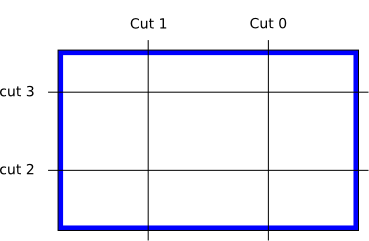
\includegraphics[scale=0.42,angle=0]{afsnit/vores_implementation/billeder/naiv_algoritme/Cut}
    \caption[]{Billedets højde og bredde betegnes hvv. $H$ og $B$. De
    fire snit er navngivet.}
    \label{cut}
\end{figure}

Indtil videre har vi kun betragtet det gyldne snit, men andre snit i
billedet kan også undersøges. Vi indfører en ny betegnelse, kaldet
\textbf{snitratio}, som beskriver hvor vi deler billedet.

\begin{definition}
	En \textbf{snitratio} er en procentsats, som multipliceret med $B$ eller
	$H$, finder placeringen af et snit i billedet.
\end{definition}

Det vil sige, hvis en snitratio er på $0.2$ i et billede med $B =
4000$, vil et snit befinde sig på pixel $4000 \cdot 0.2 = 800$ fra højre side af
billedet. Endvidere vil det samme antal pixel, fra venstre side, også være et snit.
Samme metode kan bruges på $H$ for at få to snit mere. Dette leder til
den følgende definition.

\begin{definition}
	For hver snitratio er der fire snit; to i det vertikale plan og to i
	det horisontale plan, som de røde streger illustrerer i figur
    \ref{lenasnit2}. Hvis snitratioen er lig $0.5$, findes der kun to
    snit i billedet.
\end{definition}

Hvis snitratioen er $0.5$, kommer snittene til at ligge over på hinanden,
og derved vil snitratioen kun have to snit, som vist i figur \ref{2Cut}.

\begin{figure}[!h]
    \centering
    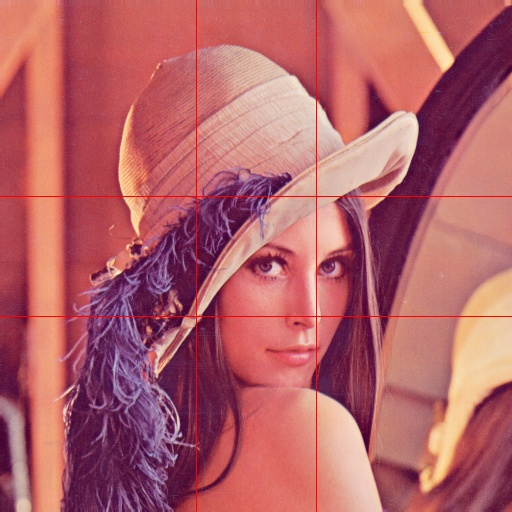
\includegraphics[scale=0.42,angle=0]{afsnit/vores_implementation/billeder/naiv_algoritme/Lenagolden}
    \caption[]{Billede, som har indtegnet de fire gyldne snit som røde
    streger.}
    \label{lenasnit2}
\end{figure}

De fire snit får tildelt hver deres Id i mændgen $\{0,1,2,3\}$. Således
kan vi skelne de enkelte snit fra hinanden. De enkelte snit navngives
som vist i figur \ref{cut}. Vi vil i fremover referere til et snit ved
dets Id.

\begin{definition}
    Hvert snit tilknyttet en snitratio, får tildelt et fast Id, som, alt
    efter snittets placering, tilhører mængden $\{0,1,2,3\}$.
\end{definition}

\begin{figure}[h]
    \centering
    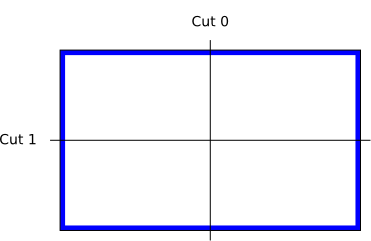
\includegraphics[scale=0.42,angle=0]{afsnit/vores_implementation/billeder/naiv_algoritme/2Cut}
    \caption[]{Snitratioen $0.5$ deler kun billedet i to snit.}
    \label{2Cut}
\end{figure}

\subsection{Acceptabel afvigelse}
Som beskrevet i afsnit \ref{mange_tal}, udregnes det gyldne snit med
mange decimaler. En kunstner, hvor god han end er, har ingen chance for
at male så præcist, at man kan sige at strøget ligger nøjagtigt oven på
snittet, selvom hans intentioner er at ramme snittet. Vi kommer derfor
til at have en vis usikkerhed på de data vi får fra billedet. Vi starter
med at se på alle de ting, som kan skabe en usikkerhed fra malerens
side. Man må gå ud fra, at den procentvise afvigelse ikke er særlig
stor, da vi ikke har bestræbelser på at arbejde på abstrakte malerier.
Vi sætter derfor den procentvise afvigelse til $0.5 \%$. Det vil sige,
at en maler med et lærred på 100 cm, maksimalt vil male $0.5$ cm
forkert.

Når maleren vælger en ramme og et lærred, har vi igen problematikken.
Selvom maleren specifikt går efter at bygge maleriet op efter det gyldne
snit, kan snittets placering i maleriet have forskubbet sig, ved dårlige
valg at ramme eller lærred. Derfor sætter vi den afvigelse til $1\%$, da
vi anser dette som den maksimale afvigelse, der kan opstå.

Når maleren maler en region i et maleri, forekommer der normalt en
lille kant rundt om objektet, et omrids. Dette omrids kan vores
algoritmer ikke tage højde for, og vi må derfor modregne omridset, så vi
er sikre på at vi ser på regionen og ikke dens omrids. Da et omrids ikke
er særligt stort, har vi sat denne procentsats til $0.5\%$.

Sammenlagt giver det en afvigelse på $2\%$. Hvis vi finder vi en region,
som ligger på pixel 200, i et billede som er $500$ cm bredt, befinder
den sig faktisk i intervallet $[190,210]$. Vi definerer derfor et
\textbf{margin} som beskriver dette.

\begin{definition}
    Hvert snit har et \textbf{margin}, som er en udvidelse af snittets
    bredde. Et margin repræsenteres som to parallelle linjer, på hver
    side af snittet, med samme afstand $\delta$ til dette.  I figur
    \ref{margin} er margin indtegnet som to blå stiplede linjer og
    snittet med rød.
\end{definition}

\begin{figure}[hb]
    \setlength\fboxsep{0pt}
    \setlength\fboxrule{0.5pt}
    \centering
    \fbox{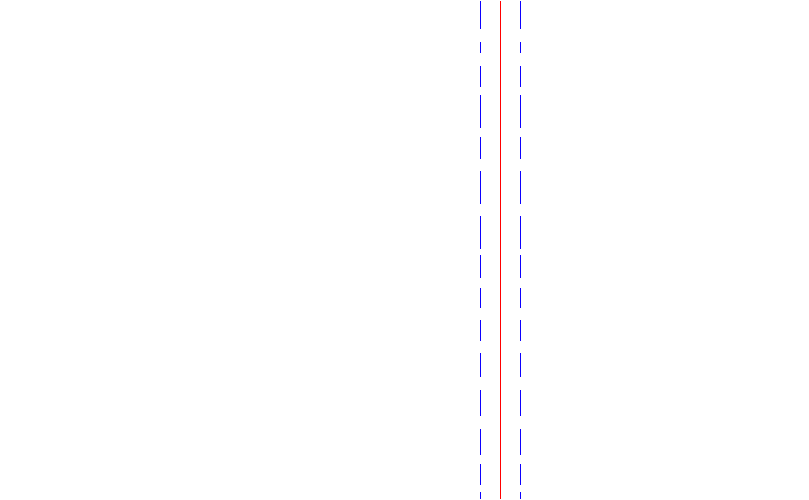
\includegraphics[scale=0.30,angle=0]{afsnit/vores_implementation/billeder/naiv_algoritme/margin.png}}
    \caption[]{snittet er den røde linie, margine er de to blå stiplet linier}
    \label{margin}
\end{figure}

Usikkerheden på $2\%$ stemmer også overens, med den usikkerhed
på $\varPhi$, som George Markowsky bruger\cite{Markowsky1992}.

\subsection{Heltal i det gyldne snit}
Vi udregner, hvor det gyldne snit er placeret, i et billede med $H =
4000$, som vist i ligning \eqref{afrundning}, hvor vi approksimerer
antal pixels, ved at afrunde resultatet $2472.13595 \approx 2472$.

\begin{equation}
    4000 \cdot \varPhi = 4000(\sqrt{5}-1)/2 = 2472.13595 \approx 2472 \label{afrundning}
\end{equation}

Ifølge udregningen i \eqref{afrundning2} betyder det, at vi mister
$0.13595$ pixels i præcision, hvilket svarer til en misvisning af
punktet på $0.00339875\%$ i forholdt til $H$.

\begin{equation}
    0.13595/4000 \cdot 100 = 0.00339875 \label{afrundning2}
\end{equation}

Det er en meget lille del af selve billedet og skulle ikke give nogle
misvisninger i forhold til udregningen. Vi sætter vores trunkeringsfejl
til $0.5$, da det er den maksimale afrundingsfaktor der kan forekomme.
Hvis billedet har en størrelse på 500 pixels, hvilket er det mindste
billede vi har, giver dette en fejlmargin på $0.1 \%$. Dette tal bliver
adderet til fejlsatsen ovenfor, og giver en samlet afvigelse på $2.1\%$.

\subsection{Heltal ved udregning af margin}
Når vi vil sammenligne regioner fra to snitratioer,  som
ligger meget tæt på hinanden --- f. eks.  $\varPhi$ og $\frac{2}{3}$ ---
er det vigtigt, at disse to snits margin ikke overlapper.

Hvis margin overlapper, vil det betyde, at den samme region kan blive
fundet i begge snit. Dette vil give et skævt billedet af regionerne i de
to snit.  I udregning \ref{diff_snit} lader vi derfor $x$ betegne
antal pixels i $B$ eller $H$, og vi vil se på, hvor mange pixels, der er
mellem snitratio $\frac{2}{3}$ og $\varPhi$, multiplicerer vi $x$ med de
to snitratioer for at finde deres placering.  Derefter subtraherer vi et
af de snit, som befinder sig tættest på hinanden, i hver snitratio med
hinanden.

\begin{eqnarray}
	\frac{x2}{3} - \frac{x2}{\sqrt{5}+1} & = & x(\frac{2}{3} - \frac{2}{\sqrt{5} + 1}) \nonumber \\
	& = & x(0.666667-0.618034) \\ \nonumber
	& = & x(0.048633)
    \label{diff_snit}
\end{eqnarray}

Vi har nu fundet antal pixel mellem de to snit. I udregning
\ref{find_Delta} finder vi den procentsats $\Delta$ for margin, som gør,
at de to margin ikke krydser hinanden, ved at dividere afstanden mellem
snitratioerne med $2$.

\begin{equation}
    \Delta = \frac{0.048633}{2} = 0.024316
    \label{find_Delta}
\end{equation}

Vi kan nu finde størrelsen på margin i pixels, som vi angiver som
$\delta$, ved at gange snittets placering $x$ på $\Delta$ og afrunde
værdien som vist i udregning \ref{marginstoerlse}.

\begin{equation}
	\delta = \left\lfloor x\Delta \right\rfloor
    \label{marginstoerlse}
\end{equation}

Den maksimale værdi af $\Delta$, når vi sammenligner det gyldne snit og
$\frac{2}{3}$, er altså $2.4316$. Det betyder også, at vi ikke kan
sammenligne snit, som ligger særlig meget tættere på hinanden, da
$2.1\%$ er den minimale værdi for $\Delta$.

\begin{definition}
    Margins størrelse i et snit, må ikke overstige $2.4316 \%$, af det
    respektive maleri $B$ eller $H$.
	\label{margin_max}
\end{definition}

\begin{definition}
	Margins størrelse i et snit, må ikke kommer under $2.1 \%$, af det
    respektive maleri $B$ eller $H$.
	\label{margin_min}
\end{definition}

Som følge af definition \ref{margin_max} og \ref{margin_min} har vi, at
$\Delta \in [0.021, 0.024316]$.

For at vise, hvor stor margin kan være i praksis, bruger vi formel
\ref{marginstoerlse} på to billeder; et, som svarer til et lille
billede, på 500 pixels, og et, som svarer til et stort billede, på 4000
pixels.  Vi sætter $\Delta = 0.024316$.  Ved 500 pixels bliver
resultatet.
\begin{equation}
	 \delta = \lfloor 500(0.024316)\rfloor = 12
\end{equation}

Det er en fin margin, da vores fejl på udregningerne ligger på $2.1\%$,
som svarer til $\lceil 500 \cdot 0.021 \rceil = 11$ pixels. Der er 1 pixel fra
vores margin.

Ved 4000 pixels giver får vi
\begin{equation}
	 \delta = \left\lfloor 4000(0.024316)\right\rfloor = 97
\end{equation}

Ovenstående er også er god nok, da $4000 \cdot 0.021 = 84$ pixels.

\clearpage
}
% vim: set tw=72 spell spelllang=da:
